\chapter{Methodology and Research Design}
\label{chap:methodology}

\section{Overview of the Proposed Framework}
\paragraph{} The proposed framework is an evidence-graded Agentic RAG pipeline for trustworthy document intelligence. The system is implemented as a full-stack prototype, but the methodology is framed as a research design. The pipeline has two stages: document representation and question answering. The document representation stage creates an uncertainty-aware document store. The question-answering stage uses query planning, structured lookup, retrieval, evidence grading, and grounded generation.

\begin{figure}[h]
\centering
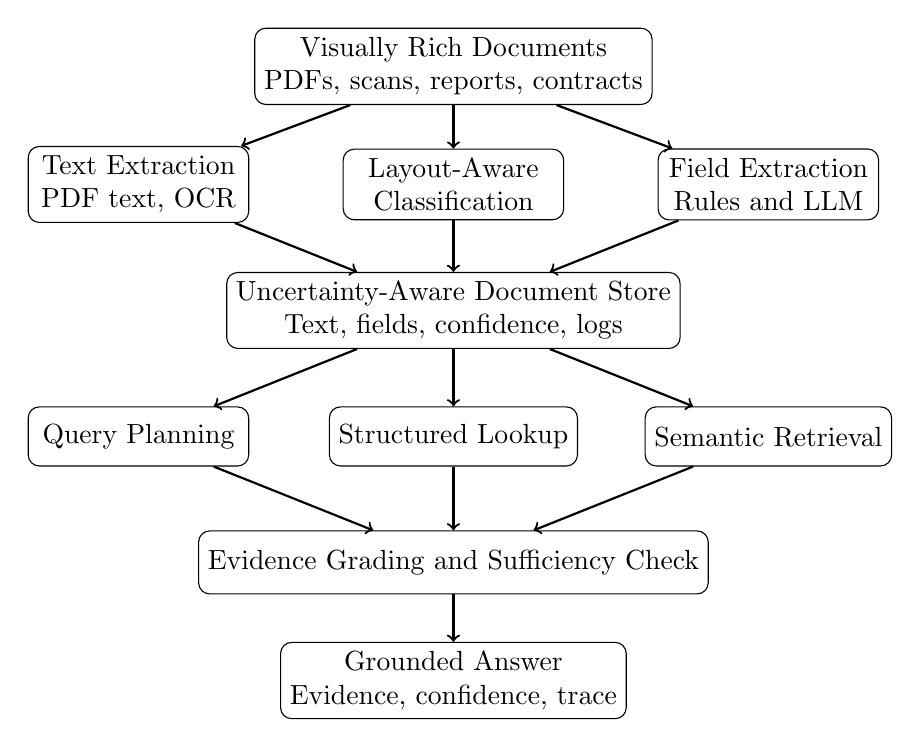
\begin{tikzpicture}[
    block/.style={rectangle, draw, rounded corners, align=center, minimum width=3.2cm, minimum height=0.8cm},
    smallblock/.style={rectangle, draw, rounded corners, align=center, minimum width=2.8cm, minimum height=0.75cm},
    arrow/.style={->, thick}
]
\node[block] (input) at (0,0) {Visually Rich Documents\\PDFs, scans, reports, contracts};
\node[smallblock] (ocr) at (-4,-1.5) {Text Extraction\\PDF text, OCR};
\node[smallblock] (layout) at (0,-1.5) {Layout-Aware\\Classification};
\node[smallblock] (fields) at (4,-1.5) {Field Extraction\\Rules and LLM};
\node[block] (store) at (0,-3.1) {Uncertainty-Aware Document Store\\Text, fields, confidence, logs};
\node[smallblock] (plan) at (-4,-4.7) {Query Planning};
\node[smallblock] (lookup) at (0,-4.7) {Structured Lookup};
\node[smallblock] (retrieve) at (4,-4.7) {Semantic Retrieval};
\node[block] (grade) at (0,-6.3) {Evidence Grading and Sufficiency Check};
\node[block] (answer) at (0,-7.8) {Grounded Answer\\Evidence, confidence, trace};

\draw[arrow] (input) -- (ocr);
\draw[arrow] (input) -- (layout);
\draw[arrow] (input) -- (fields);
\draw[arrow] (ocr) -- (store);
\draw[arrow] (layout) -- (store);
\draw[arrow] (fields) -- (store);
\draw[arrow] (store) -- (plan);
\draw[arrow] (store) -- (lookup);
\draw[arrow] (store) -- (retrieve);
\draw[arrow] (plan) -- (grade);
\draw[arrow] (lookup) -- (grade);
\draw[arrow] (retrieve) -- (grade);
\draw[arrow] (grade) -- (answer);
\end{tikzpicture}
\caption{Research framework for uncertainty-aware and evidence-graded document QA}
\label{fig:architecture}
\end{figure}

\section{Research Prototype}
\paragraph{} The prototype uses a React frontend and FastAPI backend. SQLite stores documents, extracted fields, confidence values, review flags, full text, processing logs, and chat history. The backend exposes API endpoints for upload, reprocessing, validation, search, statistics, evaluation, and Agentic RAG. The implemented system allows research experiments to be run against a real application rather than isolated notebooks.

\section{Document Representation Stage}
\paragraph{} The first stage transforms an uploaded file into an uncertainty-aware representation. Digital PDFs are processed using embedded text extraction. Scanned documents are processed using OCR. LayoutLMv3 is used for document type classification and layout-aware feature extraction. Rule-based and LLM-assisted extraction identify structured fields. Validation rules then flag suspicious values.

\paragraph{} The important research decision is to store not only final text, but also metadata that can influence downstream trust: document type, extraction confidence, source, page number, validation status, review flag, processing time, and logs. This enables later experiments on whether downstream QA improves when these uncertainty signals are used.

\begin{algorithm}[h]
\caption{Uncertainty-Aware Document Representation}
\label{alg:document_pipeline}
\begin{algorithmic}[1]
\State Receive uploaded document and create metadata record
\State Detect digital PDF or scanned-document path
\If{digital text is available}
    \State Extract embedded text directly
    \State Classify first page using layout-aware model
\Else
    \State Convert pages to images
    \State Extract OCR text and word confidence
    \State Classify pages and document type using layout-aware model
\EndIf
\State Merge page text and table text
\State Extract structured fields using rules and optional LLM extraction
\State Store field confidence and source
\State Validate fields using domain rules
\State Mark uncertain fields for review
\State Index document chunks for retrieval
\end{algorithmic}
\end{algorithm}

\section{Question Answering Stage}
\paragraph{} The second stage answers user questions. A direct RAG system would retrieve chunks and immediately ask a language model to generate an answer. The proposed workflow inserts three additional research mechanisms: intent-aware query planning, structured-field lookup, and evidence grading.

\paragraph{} Query planning classifies the question into intents such as field lookup, summary, comparison, risk review, or grounded QA. Structured-field lookup is used when the question asks for an exact extracted field such as invoice number, contract parties, amount, or date. If structured lookup fails, the system retrieves semantic chunks, grades evidence, and only then asks the language model to answer.

\begin{algorithm}[h]
\caption{Evidence-Graded Agentic RAG}
\label{alg:agentic_rag}
\begin{algorithmic}[1]
\State Receive question and optional document filter
\State Detect query intent and possible target field
\If{question can be answered from structured fields}
    \State Return structured answer with extraction confidence and evidence
\Else
    \State Retrieve candidate chunks using semantic search
    \State Score each evidence item using similarity, term coverage, and intent match
    \State Select top evidence items above sufficiency threshold
    \If{evidence is insufficient}
        \State Return insufficient-evidence response
    \Else
        \State Generate answer using selected evidence only
        \State Return answer, evidence, confidence, trace, and latency
    \EndIf
\EndIf
\end{algorithmic}
\end{algorithm}

\section{Baseline Systems}
\paragraph{} A research-centric evaluation requires baselines. The following baselines are defined for comparison:

\begin{enumerate}
    \item \textbf{B0: OCR-only extraction}: extract text and apply rule-based fields without semantic retrieval.
    \item \textbf{B1: Direct OCR plus RAG}: retrieve chunks from OCR/full text and generate an answer without structured lookup or evidence grading.
    \item \textbf{B2: Structured extraction plus direct RAG}: use structured fields for display, but answer questions through direct RAG.
    \item \textbf{B3: Proposed evidence-graded Agentic RAG}: use planning, structured lookup, retrieval, evidence grading, and sufficiency thresholding.
\end{enumerate}

\paragraph{} Comparing these baselines allows the thesis to test the value of each added component rather than only reporting final application behaviour.

\section{Variables and Metrics}
\paragraph{} The independent variable is the QA strategy: OCR-only, direct RAG, structured extraction plus RAG, or evidence-graded Agentic RAG. Dependent variables include extraction F1, retrieval precision, answer faithfulness, unsupported-claim rate, latency, throughput, and review rate.

\begin{table}[h]
\centering
\begin{tabular}{lll}
\toprule
\textbf{Metric} & \textbf{Purpose} & \textbf{Research Question} \\
\midrule
Extraction F1 & Measures key-field extraction quality & RQ1 \\
Precision@5 & Measures retrieval ranking quality & RQ3 \\
MRR & Measures first relevant result rank & RQ3 \\
Faithfulness & Measures answer support in evidence & RQ3, RQ4 \\
Unsupported-claim rate & Measures hallucination risk & RQ3, RQ4 \\
Latency & Measures user-facing efficiency & RQ2, RQ4 \\
Review rate & Measures human verification burden & RQ1, RQ4 \\
\bottomrule
\end{tabular}
\caption{Research metrics for trustworthy document intelligence}
\label{tab:technology_stack}
\end{table}

\section{System Implementation}
\paragraph{} The backend implements modular services for OCR, layout-aware classification, fusion, entity extraction, validation, search, semantic retrieval, RAG, Agentic RAG, and evaluation. The frontend provides pages for dashboard monitoring, upload, document review, search, and Agentic RAG. The application can serve the built frontend from FastAPI, making it a single runnable prototype for demonstration and evaluation.

\section{Threats to Validity}
\paragraph{} The main internal validity threat is that current heuristics may overfit to the small pilot dataset. The main external validity threat is that business documents vary widely across domains. Construct validity may be affected if automatic faithfulness metrics do not fully match human judgement. To reduce these threats, future work should use a larger document corpus, multiple annotators, held-out document templates, and both automatic and human evaluation.

\section{Reproducibility}
\paragraph{} The research prototype is organised into separate frontend, backend, service, model, and evaluation modules. The evaluation endpoint exposes computed metrics, and the API design allows repeated testing over uploaded documents. For a PhD continuation, the benchmark data, prompts, retrieved evidence, generated answers, and human labels should be stored as versioned experiment artifacts.
